\documentclass[11pt]{article}

    \usepackage[breakable]{tcolorbox}
    \usepackage{parskip} % Stop auto-indenting (to mimic markdown behaviour)
    
    \usepackage{iftex}
    \ifPDFTeX
    	\usepackage[T1]{fontenc}
    	\usepackage{mathpazo}
    \else
    	\usepackage{fontspec}
    \fi

    % Basic figure setup, for now with no caption control since it's done
    % automatically by Pandoc (which extracts ![](path) syntax from Markdown).
    \usepackage{graphicx}
    % Maintain compatibility with old templates. Remove in nbconvert 6.0
    \let\Oldincludegraphics\includegraphics
    % Ensure that by default, figures have no caption (until we provide a
    % proper Figure object with a Caption API and a way to capture that
    % in the conversion process - todo).
    \usepackage{caption}
    \DeclareCaptionFormat{nocaption}{}
    \captionsetup{format=nocaption,aboveskip=0pt,belowskip=0pt}

    \usepackage[Export]{adjustbox} % Used to constrain images to a maximum size
    \adjustboxset{max size={0.9\linewidth}{0.9\paperheight}}
    \usepackage{float}
    \floatplacement{figure}{H} % forces figures to be placed at the correct location
    \usepackage{xcolor} % Allow colors to be defined
    \usepackage{enumerate} % Needed for markdown enumerations to work
    \usepackage{geometry} % Used to adjust the document margins
    \usepackage{amsmath} % Equations
    \usepackage{amssymb} % Equations
    \usepackage{textcomp} % defines textquotesingle
    % Hack from http://tex.stackexchange.com/a/47451/13684:
    \AtBeginDocument{%
        \def\PYZsq{\textquotesingle}% Upright quotes in Pygmentized code
    }
    \usepackage{upquote} % Upright quotes for verbatim code
    \usepackage{eurosym} % defines \euro
    \usepackage[mathletters]{ucs} % Extended unicode (utf-8) support
    \usepackage{fancyvrb} % verbatim replacement that allows latex

    % The hyperref package gives us a pdf with properly built
    % internal navigation ('pdf bookmarks' for the table of contents,
    % internal cross-reference links, web links for URLs, etc.)
    \usepackage{hyperref}
    % The default LaTeX title has an obnoxious amount of whitespace. By default,
    % titling removes some of it. It also provides customization options.
    \usepackage{titling}
    \usepackage{longtable} % longtable support required by pandoc >1.10
    \usepackage{booktabs}  % table support for pandoc > 1.12.2
    \usepackage[inline]{enumitem} % IRkernel/repr support (it uses the enumerate* environment)
    \usepackage[normalem]{ulem} % ulem is needed to support strikethroughs (\sout)
                                % normalem makes italics be italics, not underlines
    \usepackage{mathrsfs}
    

    
    % Colors for the hyperref package
    \definecolor{urlcolor}{rgb}{0,.145,.698}
    \definecolor{linkcolor}{rgb}{.71,0.21,0.01}
    \definecolor{citecolor}{rgb}{.12,.54,.11}

    % ANSI colors
    \definecolor{ansi-black}{HTML}{3E424D}
    \definecolor{ansi-black-intense}{HTML}{282C36}
    \definecolor{ansi-red}{HTML}{E75C58}
    \definecolor{ansi-red-intense}{HTML}{B22B31}
    \definecolor{ansi-green}{HTML}{00A250}
    \definecolor{ansi-green-intense}{HTML}{007427}
    \definecolor{ansi-yellow}{HTML}{DDB62B}
    \definecolor{ansi-yellow-intense}{HTML}{B27D12}
    \definecolor{ansi-blue}{HTML}{208FFB}
    \definecolor{ansi-blue-intense}{HTML}{0065CA}
    \definecolor{ansi-magenta}{HTML}{D160C4}
    \definecolor{ansi-magenta-intense}{HTML}{A03196}
    \definecolor{ansi-cyan}{HTML}{60C6C8}
    \definecolor{ansi-cyan-intense}{HTML}{258F8F}
    \definecolor{ansi-white}{HTML}{C5C1B4}
    \definecolor{ansi-white-intense}{HTML}{A1A6B2}
    \definecolor{ansi-default-inverse-fg}{HTML}{FFFFFF}
    \definecolor{ansi-default-inverse-bg}{HTML}{000000}

    % commands and environments needed by pandoc snippets
    % extracted from the output of `pandoc -s`
    \providecommand{\tightlist}{%
      \setlength{\itemsep}{0pt}\setlength{\parskip}{0pt}}
    \DefineVerbatimEnvironment{Highlighting}{Verbatim}{commandchars=\\\{\}}
    % Add ',fontsize=\small' for more characters per line
    \newenvironment{Shaded}{}{}
    \newcommand{\KeywordTok}[1]{\textcolor[rgb]{0.00,0.44,0.13}{\textbf{{#1}}}}
    \newcommand{\DataTypeTok}[1]{\textcolor[rgb]{0.56,0.13,0.00}{{#1}}}
    \newcommand{\DecValTok}[1]{\textcolor[rgb]{0.25,0.63,0.44}{{#1}}}
    \newcommand{\BaseNTok}[1]{\textcolor[rgb]{0.25,0.63,0.44}{{#1}}}
    \newcommand{\FloatTok}[1]{\textcolor[rgb]{0.25,0.63,0.44}{{#1}}}
    \newcommand{\CharTok}[1]{\textcolor[rgb]{0.25,0.44,0.63}{{#1}}}
    \newcommand{\StringTok}[1]{\textcolor[rgb]{0.25,0.44,0.63}{{#1}}}
    \newcommand{\CommentTok}[1]{\textcolor[rgb]{0.38,0.63,0.69}{\textit{{#1}}}}
    \newcommand{\OtherTok}[1]{\textcolor[rgb]{0.00,0.44,0.13}{{#1}}}
    \newcommand{\AlertTok}[1]{\textcolor[rgb]{1.00,0.00,0.00}{\textbf{{#1}}}}
    \newcommand{\FunctionTok}[1]{\textcolor[rgb]{0.02,0.16,0.49}{{#1}}}
    \newcommand{\RegionMarkerTok}[1]{{#1}}
    \newcommand{\ErrorTok}[1]{\textcolor[rgb]{1.00,0.00,0.00}{\textbf{{#1}}}}
    \newcommand{\NormalTok}[1]{{#1}}
    
    % Additional commands for more recent versions of Pandoc
    \newcommand{\ConstantTok}[1]{\textcolor[rgb]{0.53,0.00,0.00}{{#1}}}
    \newcommand{\SpecialCharTok}[1]{\textcolor[rgb]{0.25,0.44,0.63}{{#1}}}
    \newcommand{\VerbatimStringTok}[1]{\textcolor[rgb]{0.25,0.44,0.63}{{#1}}}
    \newcommand{\SpecialStringTok}[1]{\textcolor[rgb]{0.73,0.40,0.53}{{#1}}}
    \newcommand{\ImportTok}[1]{{#1}}
    \newcommand{\DocumentationTok}[1]{\textcolor[rgb]{0.73,0.13,0.13}{\textit{{#1}}}}
    \newcommand{\AnnotationTok}[1]{\textcolor[rgb]{0.38,0.63,0.69}{\textbf{\textit{{#1}}}}}
    \newcommand{\CommentVarTok}[1]{\textcolor[rgb]{0.38,0.63,0.69}{\textbf{\textit{{#1}}}}}
    \newcommand{\VariableTok}[1]{\textcolor[rgb]{0.10,0.09,0.49}{{#1}}}
    \newcommand{\ControlFlowTok}[1]{\textcolor[rgb]{0.00,0.44,0.13}{\textbf{{#1}}}}
    \newcommand{\OperatorTok}[1]{\textcolor[rgb]{0.40,0.40,0.40}{{#1}}}
    \newcommand{\BuiltInTok}[1]{{#1}}
    \newcommand{\ExtensionTok}[1]{{#1}}
    \newcommand{\PreprocessorTok}[1]{\textcolor[rgb]{0.74,0.48,0.00}{{#1}}}
    \newcommand{\AttributeTok}[1]{\textcolor[rgb]{0.49,0.56,0.16}{{#1}}}
    \newcommand{\InformationTok}[1]{\textcolor[rgb]{0.38,0.63,0.69}{\textbf{\textit{{#1}}}}}
    \newcommand{\WarningTok}[1]{\textcolor[rgb]{0.38,0.63,0.69}{\textbf{\textit{{#1}}}}}
    
    
    % Define a nice break command that doesn't care if a line doesn't already
    % exist.
    \def\br{\hspace*{\fill} \\* }
    % Math Jax compatibility definitions
    \def\gt{>}
    \def\lt{<}
    \let\Oldtex\TeX
    \let\Oldlatex\LaTeX
    \renewcommand{\TeX}{\textrm{\Oldtex}}
    \renewcommand{\LaTeX}{\textrm{\Oldlatex}}
    % Document parameters
    % Document title
    \title{Lab3\_UtkarshGupta\_8PuzzleSinglePlayerGame(AStar)}
    
    
    
    
    
% Pygments definitions
\makeatletter
\def\PY@reset{\let\PY@it=\relax \let\PY@bf=\relax%
    \let\PY@ul=\relax \let\PY@tc=\relax%
    \let\PY@bc=\relax \let\PY@ff=\relax}
\def\PY@tok#1{\csname PY@tok@#1\endcsname}
\def\PY@toks#1+{\ifx\relax#1\empty\else%
    \PY@tok{#1}\expandafter\PY@toks\fi}
\def\PY@do#1{\PY@bc{\PY@tc{\PY@ul{%
    \PY@it{\PY@bf{\PY@ff{#1}}}}}}}
\def\PY#1#2{\PY@reset\PY@toks#1+\relax+\PY@do{#2}}

\expandafter\def\csname PY@tok@w\endcsname{\def\PY@tc##1{\textcolor[rgb]{0.73,0.73,0.73}{##1}}}
\expandafter\def\csname PY@tok@c\endcsname{\let\PY@it=\textit\def\PY@tc##1{\textcolor[rgb]{0.25,0.50,0.50}{##1}}}
\expandafter\def\csname PY@tok@cp\endcsname{\def\PY@tc##1{\textcolor[rgb]{0.74,0.48,0.00}{##1}}}
\expandafter\def\csname PY@tok@k\endcsname{\let\PY@bf=\textbf\def\PY@tc##1{\textcolor[rgb]{0.00,0.50,0.00}{##1}}}
\expandafter\def\csname PY@tok@kp\endcsname{\def\PY@tc##1{\textcolor[rgb]{0.00,0.50,0.00}{##1}}}
\expandafter\def\csname PY@tok@kt\endcsname{\def\PY@tc##1{\textcolor[rgb]{0.69,0.00,0.25}{##1}}}
\expandafter\def\csname PY@tok@o\endcsname{\def\PY@tc##1{\textcolor[rgb]{0.40,0.40,0.40}{##1}}}
\expandafter\def\csname PY@tok@ow\endcsname{\let\PY@bf=\textbf\def\PY@tc##1{\textcolor[rgb]{0.67,0.13,1.00}{##1}}}
\expandafter\def\csname PY@tok@nb\endcsname{\def\PY@tc##1{\textcolor[rgb]{0.00,0.50,0.00}{##1}}}
\expandafter\def\csname PY@tok@nf\endcsname{\def\PY@tc##1{\textcolor[rgb]{0.00,0.00,1.00}{##1}}}
\expandafter\def\csname PY@tok@nc\endcsname{\let\PY@bf=\textbf\def\PY@tc##1{\textcolor[rgb]{0.00,0.00,1.00}{##1}}}
\expandafter\def\csname PY@tok@nn\endcsname{\let\PY@bf=\textbf\def\PY@tc##1{\textcolor[rgb]{0.00,0.00,1.00}{##1}}}
\expandafter\def\csname PY@tok@ne\endcsname{\let\PY@bf=\textbf\def\PY@tc##1{\textcolor[rgb]{0.82,0.25,0.23}{##1}}}
\expandafter\def\csname PY@tok@nv\endcsname{\def\PY@tc##1{\textcolor[rgb]{0.10,0.09,0.49}{##1}}}
\expandafter\def\csname PY@tok@no\endcsname{\def\PY@tc##1{\textcolor[rgb]{0.53,0.00,0.00}{##1}}}
\expandafter\def\csname PY@tok@nl\endcsname{\def\PY@tc##1{\textcolor[rgb]{0.63,0.63,0.00}{##1}}}
\expandafter\def\csname PY@tok@ni\endcsname{\let\PY@bf=\textbf\def\PY@tc##1{\textcolor[rgb]{0.60,0.60,0.60}{##1}}}
\expandafter\def\csname PY@tok@na\endcsname{\def\PY@tc##1{\textcolor[rgb]{0.49,0.56,0.16}{##1}}}
\expandafter\def\csname PY@tok@nt\endcsname{\let\PY@bf=\textbf\def\PY@tc##1{\textcolor[rgb]{0.00,0.50,0.00}{##1}}}
\expandafter\def\csname PY@tok@nd\endcsname{\def\PY@tc##1{\textcolor[rgb]{0.67,0.13,1.00}{##1}}}
\expandafter\def\csname PY@tok@s\endcsname{\def\PY@tc##1{\textcolor[rgb]{0.73,0.13,0.13}{##1}}}
\expandafter\def\csname PY@tok@sd\endcsname{\let\PY@it=\textit\def\PY@tc##1{\textcolor[rgb]{0.73,0.13,0.13}{##1}}}
\expandafter\def\csname PY@tok@si\endcsname{\let\PY@bf=\textbf\def\PY@tc##1{\textcolor[rgb]{0.73,0.40,0.53}{##1}}}
\expandafter\def\csname PY@tok@se\endcsname{\let\PY@bf=\textbf\def\PY@tc##1{\textcolor[rgb]{0.73,0.40,0.13}{##1}}}
\expandafter\def\csname PY@tok@sr\endcsname{\def\PY@tc##1{\textcolor[rgb]{0.73,0.40,0.53}{##1}}}
\expandafter\def\csname PY@tok@ss\endcsname{\def\PY@tc##1{\textcolor[rgb]{0.10,0.09,0.49}{##1}}}
\expandafter\def\csname PY@tok@sx\endcsname{\def\PY@tc##1{\textcolor[rgb]{0.00,0.50,0.00}{##1}}}
\expandafter\def\csname PY@tok@m\endcsname{\def\PY@tc##1{\textcolor[rgb]{0.40,0.40,0.40}{##1}}}
\expandafter\def\csname PY@tok@gh\endcsname{\let\PY@bf=\textbf\def\PY@tc##1{\textcolor[rgb]{0.00,0.00,0.50}{##1}}}
\expandafter\def\csname PY@tok@gu\endcsname{\let\PY@bf=\textbf\def\PY@tc##1{\textcolor[rgb]{0.50,0.00,0.50}{##1}}}
\expandafter\def\csname PY@tok@gd\endcsname{\def\PY@tc##1{\textcolor[rgb]{0.63,0.00,0.00}{##1}}}
\expandafter\def\csname PY@tok@gi\endcsname{\def\PY@tc##1{\textcolor[rgb]{0.00,0.63,0.00}{##1}}}
\expandafter\def\csname PY@tok@gr\endcsname{\def\PY@tc##1{\textcolor[rgb]{1.00,0.00,0.00}{##1}}}
\expandafter\def\csname PY@tok@ge\endcsname{\let\PY@it=\textit}
\expandafter\def\csname PY@tok@gs\endcsname{\let\PY@bf=\textbf}
\expandafter\def\csname PY@tok@gp\endcsname{\let\PY@bf=\textbf\def\PY@tc##1{\textcolor[rgb]{0.00,0.00,0.50}{##1}}}
\expandafter\def\csname PY@tok@go\endcsname{\def\PY@tc##1{\textcolor[rgb]{0.53,0.53,0.53}{##1}}}
\expandafter\def\csname PY@tok@gt\endcsname{\def\PY@tc##1{\textcolor[rgb]{0.00,0.27,0.87}{##1}}}
\expandafter\def\csname PY@tok@err\endcsname{\def\PY@bc##1{\setlength{\fboxsep}{0pt}\fcolorbox[rgb]{1.00,0.00,0.00}{1,1,1}{\strut ##1}}}
\expandafter\def\csname PY@tok@kc\endcsname{\let\PY@bf=\textbf\def\PY@tc##1{\textcolor[rgb]{0.00,0.50,0.00}{##1}}}
\expandafter\def\csname PY@tok@kd\endcsname{\let\PY@bf=\textbf\def\PY@tc##1{\textcolor[rgb]{0.00,0.50,0.00}{##1}}}
\expandafter\def\csname PY@tok@kn\endcsname{\let\PY@bf=\textbf\def\PY@tc##1{\textcolor[rgb]{0.00,0.50,0.00}{##1}}}
\expandafter\def\csname PY@tok@kr\endcsname{\let\PY@bf=\textbf\def\PY@tc##1{\textcolor[rgb]{0.00,0.50,0.00}{##1}}}
\expandafter\def\csname PY@tok@bp\endcsname{\def\PY@tc##1{\textcolor[rgb]{0.00,0.50,0.00}{##1}}}
\expandafter\def\csname PY@tok@fm\endcsname{\def\PY@tc##1{\textcolor[rgb]{0.00,0.00,1.00}{##1}}}
\expandafter\def\csname PY@tok@vc\endcsname{\def\PY@tc##1{\textcolor[rgb]{0.10,0.09,0.49}{##1}}}
\expandafter\def\csname PY@tok@vg\endcsname{\def\PY@tc##1{\textcolor[rgb]{0.10,0.09,0.49}{##1}}}
\expandafter\def\csname PY@tok@vi\endcsname{\def\PY@tc##1{\textcolor[rgb]{0.10,0.09,0.49}{##1}}}
\expandafter\def\csname PY@tok@vm\endcsname{\def\PY@tc##1{\textcolor[rgb]{0.10,0.09,0.49}{##1}}}
\expandafter\def\csname PY@tok@sa\endcsname{\def\PY@tc##1{\textcolor[rgb]{0.73,0.13,0.13}{##1}}}
\expandafter\def\csname PY@tok@sb\endcsname{\def\PY@tc##1{\textcolor[rgb]{0.73,0.13,0.13}{##1}}}
\expandafter\def\csname PY@tok@sc\endcsname{\def\PY@tc##1{\textcolor[rgb]{0.73,0.13,0.13}{##1}}}
\expandafter\def\csname PY@tok@dl\endcsname{\def\PY@tc##1{\textcolor[rgb]{0.73,0.13,0.13}{##1}}}
\expandafter\def\csname PY@tok@s2\endcsname{\def\PY@tc##1{\textcolor[rgb]{0.73,0.13,0.13}{##1}}}
\expandafter\def\csname PY@tok@sh\endcsname{\def\PY@tc##1{\textcolor[rgb]{0.73,0.13,0.13}{##1}}}
\expandafter\def\csname PY@tok@s1\endcsname{\def\PY@tc##1{\textcolor[rgb]{0.73,0.13,0.13}{##1}}}
\expandafter\def\csname PY@tok@mb\endcsname{\def\PY@tc##1{\textcolor[rgb]{0.40,0.40,0.40}{##1}}}
\expandafter\def\csname PY@tok@mf\endcsname{\def\PY@tc##1{\textcolor[rgb]{0.40,0.40,0.40}{##1}}}
\expandafter\def\csname PY@tok@mh\endcsname{\def\PY@tc##1{\textcolor[rgb]{0.40,0.40,0.40}{##1}}}
\expandafter\def\csname PY@tok@mi\endcsname{\def\PY@tc##1{\textcolor[rgb]{0.40,0.40,0.40}{##1}}}
\expandafter\def\csname PY@tok@il\endcsname{\def\PY@tc##1{\textcolor[rgb]{0.40,0.40,0.40}{##1}}}
\expandafter\def\csname PY@tok@mo\endcsname{\def\PY@tc##1{\textcolor[rgb]{0.40,0.40,0.40}{##1}}}
\expandafter\def\csname PY@tok@ch\endcsname{\let\PY@it=\textit\def\PY@tc##1{\textcolor[rgb]{0.25,0.50,0.50}{##1}}}
\expandafter\def\csname PY@tok@cm\endcsname{\let\PY@it=\textit\def\PY@tc##1{\textcolor[rgb]{0.25,0.50,0.50}{##1}}}
\expandafter\def\csname PY@tok@cpf\endcsname{\let\PY@it=\textit\def\PY@tc##1{\textcolor[rgb]{0.25,0.50,0.50}{##1}}}
\expandafter\def\csname PY@tok@c1\endcsname{\let\PY@it=\textit\def\PY@tc##1{\textcolor[rgb]{0.25,0.50,0.50}{##1}}}
\expandafter\def\csname PY@tok@cs\endcsname{\let\PY@it=\textit\def\PY@tc##1{\textcolor[rgb]{0.25,0.50,0.50}{##1}}}

\def\PYZbs{\char`\\}
\def\PYZus{\char`\_}
\def\PYZob{\char`\{}
\def\PYZcb{\char`\}}
\def\PYZca{\char`\^}
\def\PYZam{\char`\&}
\def\PYZlt{\char`\<}
\def\PYZgt{\char`\>}
\def\PYZsh{\char`\#}
\def\PYZpc{\char`\%}
\def\PYZdl{\char`\$}
\def\PYZhy{\char`\-}
\def\PYZsq{\char`\'}
\def\PYZdq{\char`\"}
\def\PYZti{\char`\~}
% for compatibility with earlier versions
\def\PYZat{@}
\def\PYZlb{[}
\def\PYZrb{]}
\makeatother


    % For linebreaks inside Verbatim environment from package fancyvrb. 
    \makeatletter
        \newbox\Wrappedcontinuationbox 
        \newbox\Wrappedvisiblespacebox 
        \newcommand*\Wrappedvisiblespace {\textcolor{red}{\textvisiblespace}} 
        \newcommand*\Wrappedcontinuationsymbol {\textcolor{red}{\llap{\tiny$\m@th\hookrightarrow$}}} 
        \newcommand*\Wrappedcontinuationindent {3ex } 
        \newcommand*\Wrappedafterbreak {\kern\Wrappedcontinuationindent\copy\Wrappedcontinuationbox} 
        % Take advantage of the already applied Pygments mark-up to insert 
        % potential linebreaks for TeX processing. 
        %        {, <, #, %, $, ' and ": go to next line. 
        %        _, }, ^, &, >, - and ~: stay at end of broken line. 
        % Use of \textquotesingle for straight quote. 
        \newcommand*\Wrappedbreaksatspecials {% 
            \def\PYGZus{\discretionary{\char`\_}{\Wrappedafterbreak}{\char`\_}}% 
            \def\PYGZob{\discretionary{}{\Wrappedafterbreak\char`\{}{\char`\{}}% 
            \def\PYGZcb{\discretionary{\char`\}}{\Wrappedafterbreak}{\char`\}}}% 
            \def\PYGZca{\discretionary{\char`\^}{\Wrappedafterbreak}{\char`\^}}% 
            \def\PYGZam{\discretionary{\char`\&}{\Wrappedafterbreak}{\char`\&}}% 
            \def\PYGZlt{\discretionary{}{\Wrappedafterbreak\char`\<}{\char`\<}}% 
            \def\PYGZgt{\discretionary{\char`\>}{\Wrappedafterbreak}{\char`\>}}% 
            \def\PYGZsh{\discretionary{}{\Wrappedafterbreak\char`\#}{\char`\#}}% 
            \def\PYGZpc{\discretionary{}{\Wrappedafterbreak\char`\%}{\char`\%}}% 
            \def\PYGZdl{\discretionary{}{\Wrappedafterbreak\char`\$}{\char`\$}}% 
            \def\PYGZhy{\discretionary{\char`\-}{\Wrappedafterbreak}{\char`\-}}% 
            \def\PYGZsq{\discretionary{}{\Wrappedafterbreak\textquotesingle}{\textquotesingle}}% 
            \def\PYGZdq{\discretionary{}{\Wrappedafterbreak\char`\"}{\char`\"}}% 
            \def\PYGZti{\discretionary{\char`\~}{\Wrappedafterbreak}{\char`\~}}% 
        } 
        % Some characters . , ; ? ! / are not pygmentized. 
        % This macro makes them "active" and they will insert potential linebreaks 
        \newcommand*\Wrappedbreaksatpunct {% 
            \lccode`\~`\.\lowercase{\def~}{\discretionary{\hbox{\char`\.}}{\Wrappedafterbreak}{\hbox{\char`\.}}}% 
            \lccode`\~`\,\lowercase{\def~}{\discretionary{\hbox{\char`\,}}{\Wrappedafterbreak}{\hbox{\char`\,}}}% 
            \lccode`\~`\;\lowercase{\def~}{\discretionary{\hbox{\char`\;}}{\Wrappedafterbreak}{\hbox{\char`\;}}}% 
            \lccode`\~`\:\lowercase{\def~}{\discretionary{\hbox{\char`\:}}{\Wrappedafterbreak}{\hbox{\char`\:}}}% 
            \lccode`\~`\?\lowercase{\def~}{\discretionary{\hbox{\char`\?}}{\Wrappedafterbreak}{\hbox{\char`\?}}}% 
            \lccode`\~`\!\lowercase{\def~}{\discretionary{\hbox{\char`\!}}{\Wrappedafterbreak}{\hbox{\char`\!}}}% 
            \lccode`\~`\/\lowercase{\def~}{\discretionary{\hbox{\char`\/}}{\Wrappedafterbreak}{\hbox{\char`\/}}}% 
            \catcode`\.\active
            \catcode`\,\active 
            \catcode`\;\active
            \catcode`\:\active
            \catcode`\?\active
            \catcode`\!\active
            \catcode`\/\active 
            \lccode`\~`\~ 	
        }
    \makeatother

    \let\OriginalVerbatim=\Verbatim
    \makeatletter
    \renewcommand{\Verbatim}[1][1]{%
        %\parskip\z@skip
        \sbox\Wrappedcontinuationbox {\Wrappedcontinuationsymbol}%
        \sbox\Wrappedvisiblespacebox {\FV@SetupFont\Wrappedvisiblespace}%
        \def\FancyVerbFormatLine ##1{\hsize\linewidth
            \vtop{\raggedright\hyphenpenalty\z@\exhyphenpenalty\z@
                \doublehyphendemerits\z@\finalhyphendemerits\z@
                \strut ##1\strut}%
        }%
        % If the linebreak is at a space, the latter will be displayed as visible
        % space at end of first line, and a continuation symbol starts next line.
        % Stretch/shrink are however usually zero for typewriter font.
        \def\FV@Space {%
            \nobreak\hskip\z@ plus\fontdimen3\font minus\fontdimen4\font
            \discretionary{\copy\Wrappedvisiblespacebox}{\Wrappedafterbreak}
            {\kern\fontdimen2\font}%
        }%
        
        % Allow breaks at special characters using \PYG... macros.
        \Wrappedbreaksatspecials
        % Breaks at punctuation characters . , ; ? ! and / need catcode=\active 	
        \OriginalVerbatim[#1,codes*=\Wrappedbreaksatpunct]%
    }
    \makeatother

    % Exact colors from NB
    \definecolor{incolor}{HTML}{303F9F}
    \definecolor{outcolor}{HTML}{D84315}
    \definecolor{cellborder}{HTML}{CFCFCF}
    \definecolor{cellbackground}{HTML}{F7F7F7}
    
    % prompt
    \makeatletter
    \newcommand{\boxspacing}{\kern\kvtcb@left@rule\kern\kvtcb@boxsep}
    \makeatother
    \newcommand{\prompt}[4]{
        \ttfamily\llap{{\color{#2}[#3]:\hspace{3pt}#4}}\vspace{-\baselineskip}
    }
    

    
    % Prevent overflowing lines due to hard-to-break entities
    \sloppy 
    % Setup hyperref package
    \hypersetup{
      breaklinks=true,  % so long urls are correctly broken across lines
      colorlinks=true,
      urlcolor=urlcolor,
      linkcolor=linkcolor,
      citecolor=citecolor,
      }
    % Slightly bigger margins than the latex defaults
    
    \geometry{verbose,tmargin=1in,bmargin=1in,lmargin=1in,rmargin=1in}
    
    

\begin{document}
    
    \maketitle
    
    

    
    8 Puzzle Single Player Game (A* Algorithm)

    Introduction

An instance of the n-puzzle game consists of a board holding \(n^{2}-1\)
distinct movable tiles, plus an empty space. The tiles are numbers from
the set \(1,..,n^{2}-1\). For any such board, the empty space may be
legally swapped with any tile horizontally or vertically adjacent to it.
In this assignment, the blank space is going to be represented with the
number 0. Given an initial state of the board, the combinatorial search
problem is to find a sequence of moves that transitions this state to
the goal state; that is, the configuration with all tiles arranged in
ascending order \(0,1,..,n^{2}-1\) .

The search space is the set of all possible states reachable from the
initial state. The blank space may be swapped with a component in one of
the four directions \{`Up', `Down', `Left', `Right'\}, one move at a
time.

    In this 8 puzzle problem is discussed.

Given a 3×3 board with 8 tiles (every tile has one number from 1 to 8)
and one empty space. The objective is to place the numbers on tiles to
match final configuration using the empty space. We can slide four
adjacent (left, right, above and below) tiles into the empty space. For
example:

\begin{figure}
\centering
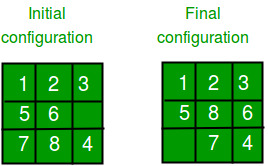
\includegraphics{puzzle8init.jpg}
\caption{alt text}
\end{figure}

    \textbf{A* Algorithm:} It is a searching algorithm that searches for the
shortest path between the initial and the final state. It is used in
various applications, such as maps. In maps the A* algorithm is used to
calculate the shortest distance between the source (initial state) and
the destination (final state).

    Explanation

A* algorithm has 3 parameters:

\begin{enumerate}
\def\labelenumi{\arabic{enumi}.}
\tightlist
\item
  g : the cost of moving from the initial cell to the current cell.
\item
  h : also known as the heuristic value, it is the estimated cost of
  moving from the current cell to the final cell. The actual cost cannot
  be calculated until the final cell is reached. Hence, h is the
  estimated cost. We must make sure that there is never an over
  estimation of the cost.
\item
  f : it is the sum of g and h. So, f = g + h
\end{enumerate}

    Example: A*

Initial State: 1, 2, 5, 3, 4, 0, 6, 7, 8

    The path to the goal node with A* (also the nodes expanded by A*) is
shown in the following figure:

    \textbf{Dear Students, in the code below there are few \emph{TODO} task
that you have to complete in this lab session.}

    \begin{tcolorbox}[breakable, size=fbox, boxrule=1pt, pad at break*=1mm,colback=cellbackground, colframe=cellborder]
\prompt{In}{incolor}{1}{\boxspacing}
\begin{Verbatim}[commandchars=\\\{\}]
\PY{k+kn}{from} \PY{n+nn}{time} \PY{k}{import} \PY{n}{time}
\PY{k+kn}{from} \PY{n+nn}{queue} \PY{k}{import} \PY{n}{PriorityQueue}
\PY{k+kn}{import} \PY{n+nn}{math}
\end{Verbatim}
\end{tcolorbox}

    \begin{tcolorbox}[breakable, size=fbox, boxrule=1pt, pad at break*=1mm,colback=cellbackground, colframe=cellborder]
\prompt{In}{incolor}{2}{\boxspacing}
\begin{Verbatim}[commandchars=\\\{\}]
\PY{c+c1}{\PYZsh{}Creating a class Puzzle}
\PY{k}{class} \PY{n+nc}{Puzzle}\PY{p}{:}
    \PY{c+c1}{\PYZsh{} Setting the goal state of 8\PYZhy{}puzzle}
    \PY{n}{goal\PYZus{}state}\PY{o}{=}\PY{p}{[}\PY{l+m+mi}{1}\PY{p}{,}\PY{l+m+mi}{2}\PY{p}{,}\PY{l+m+mi}{3}\PY{p}{,}\PY{l+m+mi}{8}\PY{p}{,}\PY{l+m+mi}{0}\PY{p}{,}\PY{l+m+mi}{4}\PY{p}{,}\PY{l+m+mi}{7}\PY{p}{,}\PY{l+m+mi}{6}\PY{p}{,}\PY{l+m+mi}{5}\PY{p}{]}
    \PY{c+c1}{\PYZsh{} Setting up the members of a class}
    \PY{n}{heuristic}\PY{o}{=}\PY{k+kc}{None}
    \PY{n}{evaluation\PYZus{}function}\PY{o}{=}\PY{k+kc}{None}
    \PY{n}{needs\PYZus{}hueristic}\PY{o}{=}\PY{k+kc}{False}
    \PY{n}{num\PYZus{}of\PYZus{}instances}\PY{o}{=}\PY{l+m+mi}{0}
    \PY{c+c1}{\PYZsh{} constructor to initialize the class members}
    \PY{k}{def} \PY{n+nf}{\PYZus{}\PYZus{}init\PYZus{}\PYZus{}}\PY{p}{(}\PY{n+nb+bp}{self}\PY{p}{,}\PY{n}{state}\PY{p}{,}\PY{n}{parent}\PY{p}{,}\PY{n}{action}\PY{p}{,}\PY{n}{path\PYZus{}cost}\PY{p}{,}\PY{n}{needs\PYZus{}hueristic}\PY{o}{=}\PY{k+kc}{False}\PY{p}{)}\PY{p}{:}
        \PY{n+nb+bp}{self}\PY{o}{.}\PY{n}{parent}\PY{o}{=}\PY{n}{parent}
        \PY{n+nb+bp}{self}\PY{o}{.}\PY{n}{state}\PY{o}{=}\PY{n}{state}
        \PY{n+nb+bp}{self}\PY{o}{.}\PY{n}{action}\PY{o}{=}\PY{n}{action}
        \PY{k}{if} \PY{n}{parent}\PY{p}{:}
            \PY{n+nb+bp}{self}\PY{o}{.}\PY{n}{path\PYZus{}cost} \PY{o}{=} \PY{n}{path\PYZus{}cost} \PY{o}{+} \PY{n}{parent}\PY{o}{.}\PY{n}{path\PYZus{}cost}
        \PY{k}{else}\PY{p}{:}
            \PY{n+nb+bp}{self}\PY{o}{.}\PY{n}{path\PYZus{}cost} \PY{o}{=} \PY{n}{path\PYZus{}cost}
        \PY{k}{if} \PY{n}{needs\PYZus{}hueristic}\PY{p}{:}
            \PY{n+nb+bp}{self}\PY{o}{.}\PY{n}{needs\PYZus{}hueristic}\PY{o}{=}\PY{k+kc}{True}
            \PY{n+nb+bp}{self}\PY{o}{.}\PY{n}{generate\PYZus{}heuristic}\PY{p}{(}\PY{p}{)}
            \PY{n+nb+bp}{self}\PY{o}{.}\PY{n}{evaluation\PYZus{}function}\PY{o}{=}\PY{n+nb+bp}{self}\PY{o}{.}\PY{n}{path\PYZus{}cost}\PY{o}{+}\PY{n+nb+bp}{self}\PY{o}{.}\PY{n}{heuristic}
        
        \PY{n}{Puzzle}\PY{o}{.}\PY{n}{num\PYZus{}of\PYZus{}instances}\PY{o}{+}\PY{o}{=} \PY{l+m+mi}{1}
    
    \PY{c+c1}{\PYZsh{} method used to display a state of 8\PYZhy{}puzzle}
    \PY{k}{def} \PY{n+nf}{\PYZus{}\PYZus{}str\PYZus{}\PYZus{}}\PY{p}{(}\PY{n+nb+bp}{self}\PY{p}{)}\PY{p}{:}
        \PY{k}{return} \PY{n+nb}{str}\PY{p}{(}\PY{n+nb+bp}{self}\PY{o}{.}\PY{n}{state}\PY{p}{[}\PY{l+m+mi}{0}\PY{p}{:}\PY{l+m+mi}{3}\PY{p}{]}\PY{p}{)}\PY{o}{+}\PY{l+s+s1}{\PYZsq{}}\PY{l+s+se}{\PYZbs{}n}\PY{l+s+s1}{\PYZsq{}}\PY{o}{+}\PY{n+nb}{str}\PY{p}{(}\PY{n+nb+bp}{self}\PY{o}{.}\PY{n}{state}\PY{p}{[}\PY{l+m+mi}{3}\PY{p}{:}\PY{l+m+mi}{6}\PY{p}{]}\PY{p}{)}\PY{o}{+}\PY{l+s+s1}{\PYZsq{}}\PY{l+s+se}{\PYZbs{}n}\PY{l+s+s1}{\PYZsq{}}\PY{o}{+}\PY{n+nb}{str}\PY{p}{(}\PY{n+nb+bp}{self}\PY{o}{.}\PY{n}{state}\PY{p}{[}\PY{l+m+mi}{6}\PY{p}{:}\PY{l+m+mi}{9}\PY{p}{]}\PY{p}{)}

    \PY{c+c1}{\PYZsh{} method used to generate a heuristic value}
    \PY{k}{def} \PY{n+nf}{generate\PYZus{}heuristic}\PY{p}{(}\PY{n+nb+bp}{self}\PY{p}{)}\PY{p}{:}
        \PY{n+nb+bp}{self}\PY{o}{.}\PY{n}{heuristic}\PY{o}{=}\PY{l+m+mi}{0}
        \PY{k}{for} \PY{n}{num} \PY{o+ow}{in} \PY{n+nb}{range}\PY{p}{(}\PY{l+m+mi}{1}\PY{p}{,}\PY{l+m+mi}{9}\PY{p}{)}\PY{p}{:}
            \PY{n}{distance}\PY{o}{=}\PY{n+nb}{abs}\PY{p}{(}\PY{n+nb+bp}{self}\PY{o}{.}\PY{n}{state}\PY{o}{.}\PY{n}{index}\PY{p}{(}\PY{n}{num}\PY{p}{)}\PY{o}{\PYZhy{}}\PY{n+nb+bp}{self}\PY{o}{.}\PY{n}{goal\PYZus{}state}\PY{o}{.}\PY{n}{index}\PY{p}{(}\PY{n}{num}\PY{p}{)}\PY{p}{)}
            \PY{n}{i}\PY{o}{=}\PY{n+nb}{int}\PY{p}{(}\PY{n}{distance}\PY{o}{/}\PY{l+m+mi}{3}\PY{p}{)}
            \PY{n}{j}\PY{o}{=}\PY{n+nb}{int}\PY{p}{(}\PY{n}{distance}\PY{o}{\PYZpc{}}\PY{k}{3})
            \PY{n+nb+bp}{self}\PY{o}{.}\PY{n}{heuristic}\PY{o}{=}\PY{n+nb+bp}{self}\PY{o}{.}\PY{n}{heuristic}\PY{o}{+}\PY{n}{i}\PY{o}{+}\PY{n}{j}

    \PY{k}{def} \PY{n+nf}{goal\PYZus{}test}\PY{p}{(}\PY{n+nb+bp}{self}\PY{p}{)}\PY{p}{:}
        \PY{k}{if} \PY{p}{(}\PY{n+nb+bp}{self}\PY{o}{.}\PY{n}{state}\PY{o}{==}\PY{n+nb+bp}{self}\PY{o}{.}\PY{n}{goal\PYZus{}state}\PY{p}{)}\PY{p}{:}
            \PY{k}{return} \PY{k+kc}{True}
        \PY{k}{return} \PY{k+kc}{False}

    \PY{n+nd}{@staticmethod}
    \PY{k}{def} \PY{n+nf}{find\PYZus{}legal\PYZus{}actions}\PY{p}{(}\PY{n}{i}\PY{p}{,}\PY{n}{j}\PY{p}{)}\PY{p}{:}
        \PY{c+c1}{\PYZsh{} find the legal actions as Up, Down, Left, Right based on each cell of state}
        \PY{n}{legal\PYZus{}action} \PY{o}{=} \PY{p}{[}\PY{l+s+s1}{\PYZsq{}}\PY{l+s+s1}{U}\PY{l+s+s1}{\PYZsq{}}\PY{p}{,} \PY{l+s+s1}{\PYZsq{}}\PY{l+s+s1}{D}\PY{l+s+s1}{\PYZsq{}}\PY{p}{,} \PY{l+s+s1}{\PYZsq{}}\PY{l+s+s1}{L}\PY{l+s+s1}{\PYZsq{}}\PY{p}{,} \PY{l+s+s1}{\PYZsq{}}\PY{l+s+s1}{R}\PY{l+s+s1}{\PYZsq{}}\PY{p}{]}
        \PY{k}{if} \PY{n}{i} \PY{o}{==} \PY{l+m+mi}{0}\PY{p}{:}  \PY{c+c1}{\PYZsh{} up is disable}
            \PY{c+c1}{\PYZsh{} if row is 0 in board then up is disable}
            \PY{n}{legal\PYZus{}action}\PY{o}{.}\PY{n}{remove}\PY{p}{(}\PY{l+s+s1}{\PYZsq{}}\PY{l+s+s1}{U}\PY{l+s+s1}{\PYZsq{}}\PY{p}{)}
        \PY{k}{elif} \PY{n}{i} \PY{o}{==} \PY{l+m+mi}{2}\PY{p}{:}
             \PY{n}{legal\PYZus{}action}\PY{o}{.}\PY{n}{remove}\PY{p}{(}\PY{l+s+s1}{\PYZsq{}}\PY{l+s+s1}{D}\PY{l+s+s1}{\PYZsq{}}\PY{p}{)}
        \PY{k}{if} \PY{n}{j} \PY{o}{==} \PY{l+m+mi}{0}\PY{p}{:}
             \PY{n}{legal\PYZus{}action}\PY{o}{.}\PY{n}{remove}\PY{p}{(}\PY{l+s+s1}{\PYZsq{}}\PY{l+s+s1}{L}\PY{l+s+s1}{\PYZsq{}}\PY{p}{)}
        \PY{k}{elif} \PY{n}{j} \PY{o}{==} \PY{l+m+mi}{2}\PY{p}{:}
             \PY{n}{legal\PYZus{}action}\PY{o}{.}\PY{n}{remove}\PY{p}{(}\PY{l+s+s1}{\PYZsq{}}\PY{l+s+s1}{R}\PY{l+s+s1}{\PYZsq{}}\PY{p}{)}
        \PY{k}{return} \PY{n}{legal\PYZus{}action}

    \PY{c+c1}{\PYZsh{} method to generate the child of the current state of the board}
    \PY{k}{def} \PY{n+nf}{generate\PYZus{}child}\PY{p}{(}\PY{n+nb+bp}{self}\PY{p}{)}\PY{p}{:}
        \PY{n}{children}\PY{o}{=}\PY{p}{[}\PY{p}{]}
        \PY{n}{x} \PY{o}{=} \PY{n+nb+bp}{self}\PY{o}{.}\PY{n}{state}\PY{o}{.}\PY{n}{index}\PY{p}{(}\PY{l+m+mi}{0}\PY{p}{)}
        \PY{n}{i} \PY{o}{=} \PY{n+nb}{int}\PY{p}{(}\PY{n}{x} \PY{o}{/} \PY{l+m+mi}{3}\PY{p}{)}
        \PY{n}{j} \PY{o}{=} \PY{n+nb}{int}\PY{p}{(}\PY{n}{x} \PY{o}{\PYZpc{}} \PY{l+m+mi}{3}\PY{p}{)}
        \PY{n}{legal\PYZus{}actions}\PY{o}{=}\PY{n+nb+bp}{self}\PY{o}{.}\PY{n}{find\PYZus{}legal\PYZus{}actions}\PY{p}{(}\PY{n}{i}\PY{p}{,}\PY{n}{j}\PY{p}{)}

        \PY{k}{for} \PY{n}{action} \PY{o+ow}{in} \PY{n}{legal\PYZus{}actions}\PY{p}{:}
            \PY{n}{new\PYZus{}state} \PY{o}{=} \PY{n+nb+bp}{self}\PY{o}{.}\PY{n}{state}\PY{o}{.}\PY{n}{copy}\PY{p}{(}\PY{p}{)}
            \PY{c+c1}{\PYZsh{} if the legal action is UP}
            \PY{k}{if} \PY{n}{action} \PY{o}{==} \PY{l+s+s1}{\PYZsq{}}\PY{l+s+s1}{U}\PY{l+s+s1}{\PYZsq{}}\PY{p}{:}
                \PY{c+c1}{\PYZsh{} Swapping between current index of 0 with its up element on the board}
                \PY{n}{new\PYZus{}state}\PY{p}{[}\PY{n}{x}\PY{p}{]}\PY{p}{,} \PY{n}{new\PYZus{}state}\PY{p}{[}\PY{n}{x}\PY{o}{\PYZhy{}}\PY{l+m+mi}{3}\PY{p}{]} \PY{o}{=} \PY{n}{new\PYZus{}state}\PY{p}{[}\PY{n}{x}\PY{o}{\PYZhy{}}\PY{l+m+mi}{3}\PY{p}{]}\PY{p}{,} \PY{n}{new\PYZus{}state}\PY{p}{[}\PY{n}{x}\PY{p}{]}
            \PY{k}{elif} \PY{n}{action} \PY{o}{==} \PY{l+s+s1}{\PYZsq{}}\PY{l+s+s1}{D}\PY{l+s+s1}{\PYZsq{}}\PY{p}{:}
                \PY{n}{new\PYZus{}state}\PY{p}{[}\PY{n}{x}\PY{p}{]}\PY{p}{,} \PY{n}{new\PYZus{}state}\PY{p}{[}\PY{n}{x}\PY{o}{+}\PY{l+m+mi}{3}\PY{p}{]} \PY{o}{=} \PY{n}{new\PYZus{}state}\PY{p}{[}\PY{n}{x}\PY{o}{+}\PY{l+m+mi}{3}\PY{p}{]}\PY{p}{,} \PY{n}{new\PYZus{}state}\PY{p}{[}\PY{n}{x}\PY{p}{]}
            \PY{k}{elif} \PY{n}{action} \PY{o}{==} \PY{l+s+s1}{\PYZsq{}}\PY{l+s+s1}{L}\PY{l+s+s1}{\PYZsq{}}\PY{p}{:}
                \PY{n}{new\PYZus{}state}\PY{p}{[}\PY{n}{x}\PY{p}{]}\PY{p}{,} \PY{n}{new\PYZus{}state}\PY{p}{[}\PY{n}{x}\PY{o}{\PYZhy{}}\PY{l+m+mi}{1}\PY{p}{]} \PY{o}{=} \PY{n}{new\PYZus{}state}\PY{p}{[}\PY{n}{x}\PY{o}{\PYZhy{}}\PY{l+m+mi}{1}\PY{p}{]}\PY{p}{,} \PY{n}{new\PYZus{}state}\PY{p}{[}\PY{n}{x}\PY{p}{]}
            \PY{k}{elif} \PY{n}{action} \PY{o}{==} \PY{l+s+s1}{\PYZsq{}}\PY{l+s+s1}{R}\PY{l+s+s1}{\PYZsq{}}\PY{p}{:}
                \PY{n}{new\PYZus{}state}\PY{p}{[}\PY{n}{x}\PY{p}{]}\PY{p}{,} \PY{n}{new\PYZus{}state}\PY{p}{[}\PY{n}{x}\PY{o}{+}\PY{l+m+mi}{1}\PY{p}{]} \PY{o}{=} \PY{n}{new\PYZus{}state}\PY{p}{[}\PY{n}{x}\PY{o}{+}\PY{l+m+mi}{1}\PY{p}{]}\PY{p}{,} \PY{n}{new\PYZus{}state}\PY{p}{[}\PY{n}{x}\PY{p}{]}

            \PY{n}{children}\PY{o}{.}\PY{n}{append}\PY{p}{(}\PY{n}{Puzzle}\PY{p}{(}\PY{n}{new\PYZus{}state}\PY{p}{,}\PY{n+nb+bp}{self}\PY{p}{,}\PY{n}{action}\PY{p}{,}\PY{l+m+mi}{1}\PY{p}{,}\PY{k+kc}{True}\PY{p}{)}\PY{p}{)}
        
        \PY{k}{return} \PY{n}{children}
    
    \PY{c+c1}{\PYZsh{} method to find the solution}
    \PY{k}{def} \PY{n+nf}{find\PYZus{}solution}\PY{p}{(}\PY{n+nb+bp}{self}\PY{p}{)}\PY{p}{:}
        \PY{n}{solution} \PY{o}{=} \PY{p}{[}\PY{p}{]}
        \PY{n}{solution}\PY{o}{.}\PY{n}{append}\PY{p}{(}\PY{n+nb+bp}{self}\PY{o}{.}\PY{n}{action}\PY{p}{)}
        \PY{c+c1}{\PYZsh{} implementing the Bonus Task: @utkarsh2102}
        \PY{n}{solution\PYZus{}path} \PY{o}{=} \PY{p}{[}\PY{p}{]}
        \PY{n}{solution\PYZus{}path}\PY{o}{.}\PY{n}{append}\PY{p}{(}\PY{n+nb+bp}{self}\PY{p}{)}
        \PY{n}{path} \PY{o}{=} \PY{n+nb+bp}{self}
        \PY{k}{while} \PY{n}{path}\PY{o}{.}\PY{n}{parent} \PY{o}{!=} \PY{k+kc}{None}\PY{p}{:}
            \PY{n}{path} \PY{o}{=} \PY{n}{path}\PY{o}{.}\PY{n}{parent}
            \PY{n}{solution}\PY{o}{.}\PY{n}{append}\PY{p}{(}\PY{n}{path}\PY{o}{.}\PY{n}{action}\PY{p}{)}
            \PY{n}{solution\PYZus{}path}\PY{o}{.}\PY{n}{append}\PY{p}{(}\PY{n}{path}\PY{p}{)}
        \PY{n}{solution} \PY{o}{=} \PY{n}{solution}\PY{p}{[}\PY{p}{:}\PY{o}{\PYZhy{}}\PY{l+m+mi}{1}\PY{p}{]}
        \PY{n}{solution}\PY{o}{.}\PY{n}{reverse}\PY{p}{(}\PY{p}{)}
        \PY{n}{solution\PYZus{}path}\PY{o}{.}\PY{n}{reverse}\PY{p}{(}\PY{p}{)}
        \PY{c+c1}{\PYZsh{} iterating the list to print the path as we go}
        \PY{k}{for} \PY{n}{i} \PY{o+ow}{in} \PY{n}{solution\PYZus{}path}\PY{p}{:}
          \PY{n+nb}{print}\PY{p}{(}\PY{n}{i}\PY{p}{)}
          \PY{n+nb}{print}\PY{p}{(}\PY{p}{)}
        \PY{k}{return} \PY{n}{solution}
\end{Verbatim}
\end{tcolorbox}

    \begin{tcolorbox}[breakable, size=fbox, boxrule=1pt, pad at break*=1mm,colback=cellbackground, colframe=cellborder]
\prompt{In}{incolor}{3}{\boxspacing}
\begin{Verbatim}[commandchars=\\\{\}]
\PY{c+c1}{\PYZsh{} method for A\PYZhy{}star search}
\PY{k}{def} \PY{n+nf}{Astar\PYZus{}search}\PY{p}{(}\PY{n}{initial\PYZus{}state}\PY{p}{)}\PY{p}{:}
    \PY{n}{count}\PY{o}{=}\PY{l+m+mi}{0}
    \PY{n}{explored}\PY{o}{=}\PY{p}{[}\PY{p}{]}
    \PY{n}{start\PYZus{}node}\PY{o}{=} \PY{n}{Puzzle}\PY{p}{(}\PY{n}{initial\PYZus{}state}\PY{p}{,} \PY{k+kc}{None}\PY{p}{,} \PY{k+kc}{None}\PY{p}{,} \PY{l+m+mi}{0}\PY{p}{,} \PY{k+kc}{True}\PY{p}{)}
    \PY{n+nb}{print}\PY{p}{(}\PY{l+s+s2}{\PYZdq{}}\PY{l+s+s2}{\PYZhy{}\PYZhy{}\PYZhy{}\PYZhy{}\PYZhy{}\PYZhy{}\PYZhy{}\PYZhy{}\PYZhy{}\PYZhy{}\PYZhy{}\PYZhy{}\PYZhy{}\PYZhy{}\PYZhy{}\PYZhy{}\PYZhy{}\PYZhy{}\PYZhy{}\PYZhy{}\PYZhy{}\PYZhy{}\PYZhy{}\PYZhy{}\PYZhy{}\PYZhy{}\PYZhy{}\PYZhy{}\PYZhy{}\PYZhy{}\PYZhy{}\PYZhy{}\PYZhy{}\PYZhy{}\PYZhy{}\PYZhy{}\PYZhy{}\PYZhy{}\PYZhy{}\PYZhy{}\PYZhy{}\PYZhy{}}\PY{l+s+s2}{\PYZdq{}}\PY{p}{)}
    \PY{n+nb}{print}\PY{p}{(}\PY{p}{)}
    \PY{n+nb}{print}\PY{p}{(}\PY{l+s+s2}{\PYZdq{}}\PY{l+s+s2}{Initial state:}\PY{l+s+s2}{\PYZdq{}}\PY{p}{)}
    \PY{n+nb}{print}\PY{p}{(}\PY{n}{start\PYZus{}node}\PY{p}{)}
    \PY{n+nb}{print}\PY{p}{(}\PY{p}{)}
    \PY{n+nb}{print}\PY{p}{(}\PY{l+s+s2}{\PYZdq{}}\PY{l+s+s2}{Solution path in the A\PYZhy{}star algorithm is: }\PY{l+s+s2}{\PYZdq{}}\PY{p}{)}
    \PY{n}{q} \PY{o}{=} \PY{n}{PriorityQueue}\PY{p}{(}\PY{p}{)}
    \PY{n}{q}\PY{o}{.}\PY{n}{put}\PY{p}{(}\PY{p}{(}\PY{n}{start\PYZus{}node}\PY{o}{.}\PY{n}{evaluation\PYZus{}function}\PY{p}{,} \PY{n}{count}\PY{p}{,} \PY{n}{start\PYZus{}node}\PY{p}{)}\PY{p}{)}

    \PY{k}{while} \PY{o+ow}{not} \PY{n}{q}\PY{o}{.}\PY{n}{empty}\PY{p}{(}\PY{p}{)}\PY{p}{:}
        \PY{n}{node}\PY{o}{=}\PY{n}{q}\PY{o}{.}\PY{n}{get}\PY{p}{(}\PY{p}{)}
        \PY{n}{node}\PY{o}{=}\PY{n}{node}\PY{p}{[}\PY{l+m+mi}{2}\PY{p}{]}
        \PY{n}{explored}\PY{o}{.}\PY{n}{append}\PY{p}{(}\PY{n}{node}\PY{o}{.}\PY{n}{state}\PY{p}{)}
        \PY{k}{if} \PY{n}{node}\PY{o}{.}\PY{n}{goal\PYZus{}test}\PY{p}{(}\PY{p}{)}\PY{p}{:}
            \PY{k}{return} \PY{n}{node}\PY{o}{.}\PY{n}{find\PYZus{}solution}\PY{p}{(}\PY{p}{)}

        \PY{n}{children}\PY{o}{=}\PY{n}{node}\PY{o}{.}\PY{n}{generate\PYZus{}child}\PY{p}{(}\PY{p}{)}
        \PY{k}{for} \PY{n}{child} \PY{o+ow}{in} \PY{n}{children}\PY{p}{:}
            \PY{k}{if} \PY{n}{child}\PY{o}{.}\PY{n}{state} \PY{o+ow}{not} \PY{o+ow}{in} \PY{n}{explored}\PY{p}{:}
                \PY{n}{count} \PY{o}{+}\PY{o}{=} \PY{l+m+mi}{1}
                \PY{n}{q}\PY{o}{.}\PY{n}{put}\PY{p}{(}\PY{p}{(}\PY{n}{child}\PY{o}{.}\PY{n}{evaluation\PYZus{}function}\PY{p}{,} \PY{n}{count}\PY{p}{,} \PY{n}{child}\PY{p}{)}\PY{p}{)}
    \PY{k}{return}
\end{Verbatim}
\end{tcolorbox}

    \begin{tcolorbox}[breakable, size=fbox, boxrule=1pt, pad at break*=1mm,colback=cellbackground, colframe=cellborder]
\prompt{In}{incolor}{6}{\boxspacing}
\begin{Verbatim}[commandchars=\\\{\}]
\PY{c+c1}{\PYZsh{} Start executing the 8\PYZhy{}puzzle with setting up the initial state}
\PY{c+c1}{\PYZsh{} Here we have considered 3 initial state intitalized using state variable}
\PY{n}{state}\PY{o}{=}\PY{p}{[}\PY{p}{[}\PY{l+m+mi}{1}\PY{p}{,} \PY{l+m+mi}{3}\PY{p}{,} \PY{l+m+mi}{4}\PY{p}{,}
        \PY{l+m+mi}{8}\PY{p}{,} \PY{l+m+mi}{6}\PY{p}{,} \PY{l+m+mi}{2}\PY{p}{,}
        \PY{l+m+mi}{7}\PY{p}{,} \PY{l+m+mi}{0}\PY{p}{,} \PY{l+m+mi}{5}\PY{p}{]}\PY{p}{,}

       \PY{p}{[}\PY{l+m+mi}{2}\PY{p}{,} \PY{l+m+mi}{8}\PY{p}{,} \PY{l+m+mi}{1}\PY{p}{,}
        \PY{l+m+mi}{0}\PY{p}{,} \PY{l+m+mi}{4}\PY{p}{,} \PY{l+m+mi}{3}\PY{p}{,}
        \PY{l+m+mi}{7}\PY{p}{,} \PY{l+m+mi}{6}\PY{p}{,} \PY{l+m+mi}{5}\PY{p}{]}\PY{p}{,}

       \PY{p}{[}\PY{l+m+mi}{2}\PY{p}{,} \PY{l+m+mi}{8}\PY{p}{,} \PY{l+m+mi}{1}\PY{p}{,}
        \PY{l+m+mi}{4}\PY{p}{,} \PY{l+m+mi}{6}\PY{p}{,} \PY{l+m+mi}{3}\PY{p}{,}
        \PY{l+m+mi}{0}\PY{p}{,} \PY{l+m+mi}{7}\PY{p}{,} \PY{l+m+mi}{5}\PY{p}{]}\PY{p}{]}

\PY{c+c1}{\PYZsh{} Iterate over number of initial\PYZus{}state}
\PY{k}{for} \PY{n}{i} \PY{o+ow}{in} \PY{n+nb}{range}\PY{p}{(}\PY{l+m+mi}{0}\PY{p}{,}\PY{l+m+mi}{3}\PY{p}{)}\PY{p}{:}
    \PY{n}{Puzzle}\PY{o}{.}\PY{n}{num\PYZus{}of\PYZus{}instances} \PY{o}{=} \PY{l+m+mi}{0}
    \PY{c+c1}{\PYZsh{} Set t0 to current time}
    \PY{n}{t0} \PY{o}{=} \PY{n}{time}\PY{p}{(}\PY{p}{)}
    \PY{n}{astar} \PY{o}{=} \PY{n}{Astar\PYZus{}search}\PY{p}{(}\PY{n}{state}\PY{p}{[}\PY{n}{i}\PY{p}{]}\PY{p}{)}
    \PY{c+c1}{\PYZsh{} Get the time t1 after executing the breadth\PYZus{}first\PYZus{}search method}
    \PY{n}{t1} \PY{o}{=} \PY{n}{time}\PY{p}{(}\PY{p}{)} \PY{o}{\PYZhy{}} \PY{n}{t0}
    \PY{n+nb}{print}\PY{p}{(}\PY{l+s+s2}{\PYZdq{}}\PY{l+s+s2}{A*:    }\PY{l+s+s2}{\PYZdq{}}\PY{p}{,} \PY{n}{astar}\PY{p}{)}
    \PY{n+nb}{print}\PY{p}{(}\PY{l+s+s2}{\PYZdq{}}\PY{l+s+s2}{Space: }\PY{l+s+s2}{\PYZdq{}}\PY{p}{,} \PY{n}{Puzzle}\PY{o}{.}\PY{n}{num\PYZus{}of\PYZus{}instances}\PY{p}{)}
    \PY{n+nb}{print}\PY{p}{(}\PY{l+s+s2}{\PYZdq{}}\PY{l+s+s2}{Time:  }\PY{l+s+s2}{\PYZdq{}}\PY{p}{,} \PY{n}{t1}\PY{p}{)}
    \PY{n+nb}{print}\PY{p}{(}\PY{l+s+s2}{\PYZdq{}}\PY{l+s+s2}{Bonus task done by Utkarsh Gupta (A2305217557)}\PY{l+s+s2}{\PYZdq{}}\PY{p}{)}
    \PY{n+nb}{print}\PY{p}{(}\PY{p}{)}
    \PY{n+nb}{print}\PY{p}{(}\PY{l+s+s2}{\PYZdq{}}\PY{l+s+s2}{\PYZhy{}\PYZhy{}\PYZhy{}\PYZhy{}\PYZhy{}\PYZhy{}\PYZhy{}\PYZhy{}\PYZhy{}\PYZhy{}\PYZhy{}\PYZhy{}\PYZhy{}\PYZhy{}\PYZhy{}\PYZhy{}\PYZhy{}\PYZhy{}\PYZhy{}\PYZhy{}\PYZhy{}\PYZhy{}\PYZhy{}\PYZhy{}\PYZhy{}\PYZhy{}\PYZhy{}\PYZhy{}\PYZhy{}\PYZhy{}\PYZhy{}\PYZhy{}\PYZhy{}\PYZhy{}\PYZhy{}\PYZhy{}\PYZhy{}\PYZhy{}\PYZhy{}\PYZhy{}\PYZhy{}\PYZhy{}}\PY{l+s+s2}{\PYZdq{}}\PY{p}{)}
\end{Verbatim}
\end{tcolorbox}

    \begin{Verbatim}[commandchars=\\\{\}]
------------------------------------------

Initial state:
[1, 3, 4]
[8, 6, 2]
[7, 0, 5]

Solution path in the A-star algorithm is:
[1, 3, 4]
[8, 6, 2]
[7, 0, 5]

[1, 3, 4]
[8, 0, 2]
[7, 6, 5]

[1, 3, 4]
[8, 2, 0]
[7, 6, 5]

[1, 3, 0]
[8, 2, 4]
[7, 6, 5]

[1, 0, 3]
[8, 2, 4]
[7, 6, 5]

[1, 2, 3]
[8, 0, 4]
[7, 6, 5]

A*:     ['U', 'R', 'U', 'L', 'D']
Space:  16
Time:   0.0008704662322998047
Bonus task done by Utkarsh Gupta (A2305217557)

------------------------------------------
------------------------------------------

Initial state:
[2, 8, 1]
[0, 4, 3]
[7, 6, 5]

Solution path in the A-star algorithm is:
[2, 8, 1]
[0, 4, 3]
[7, 6, 5]

[0, 8, 1]
[2, 4, 3]
[7, 6, 5]

[8, 0, 1]
[2, 4, 3]
[7, 6, 5]

[8, 1, 0]
[2, 4, 3]
[7, 6, 5]

[8, 1, 3]
[2, 4, 0]
[7, 6, 5]

[8, 1, 3]
[2, 0, 4]
[7, 6, 5]

[8, 1, 3]
[0, 2, 4]
[7, 6, 5]

[0, 1, 3]
[8, 2, 4]
[7, 6, 5]

[1, 0, 3]
[8, 2, 4]
[7, 6, 5]

[1, 2, 3]
[8, 0, 4]
[7, 6, 5]

A*:     ['U', 'R', 'R', 'D', 'L', 'L', 'U', 'R', 'D']
Space:  42
Time:   0.0008480548858642578
Bonus task done by Utkarsh Gupta (A2305217557)

------------------------------------------
------------------------------------------

Initial state:
[2, 8, 1]
[4, 6, 3]
[0, 7, 5]

Solution path in the A-star algorithm is:
[2, 8, 1]
[4, 6, 3]
[0, 7, 5]

[2, 8, 1]
[4, 6, 3]
[7, 0, 5]

[2, 8, 1]
[4, 0, 3]
[7, 6, 5]

[2, 8, 1]
[0, 4, 3]
[7, 6, 5]

[0, 8, 1]
[2, 4, 3]
[7, 6, 5]

[8, 0, 1]
[2, 4, 3]
[7, 6, 5]

[8, 1, 0]
[2, 4, 3]
[7, 6, 5]

[8, 1, 3]
[2, 4, 0]
[7, 6, 5]

[8, 1, 3]
[2, 0, 4]
[7, 6, 5]

[8, 1, 3]
[0, 2, 4]
[7, 6, 5]

[0, 1, 3]
[8, 2, 4]
[7, 6, 5]

[1, 0, 3]
[8, 2, 4]
[7, 6, 5]

[1, 2, 3]
[8, 0, 4]
[7, 6, 5]

A*:     ['R', 'U', 'L', 'U', 'R', 'R', 'D', 'L', 'L', 'U', 'R', 'D']
Space:  95
Time:   0.005315542221069336
Bonus task done by Utkarsh Gupta (A2305217557)

------------------------------------------
    \end{Verbatim}

    \textbf{BONUS TASK:} Now, perform the following task before submitting
the assignment:

Show the path in traversing the A-star algorithm of each state from
intial\_state to goal state.


    % Add a bibliography block to the postdoc
    
    
    
\end{document}
